\documentclass[11pt,oneside,a4paper,twocolumn]{article}
\usepackage{booktabs}
\usepackage{hyperref}
\usepackage[utf8]{inputenc}
\usepackage[english]{babel}
\usepackage{fancyhdr}
\usepackage{graphicx}
\usepackage{parskip}
\usepackage[affil-it]{authblk}
\usepackage{lipsum}
\usepackage[sorting=none]{biblatex}
\usepackage{csquotes}
\usepackage{multirow}
\usepackage[table,xcdraw]{xcolor}
\usepackage{rotating}
\usepackage{enumitem}
\usepackage{subcaption}
\usepackage{caption}

\setlength{\headheight}{14pt}


\addbibresource{bibliography.bib}



\makeatletter
\def\thm@space@setup{%
  \thm@preskip=\parskip \thm@postskip=0pt
}

\pagestyle{fancy}

\title{Painting Detection and Rectification with People Detection}

\author{Aniello Panariello - 140195}
\author{Fabrizio Sorgente - 133855}
\author{Emanuele Fenocchi - 148869}
\affil{University of Modena and Reggio Emilia}

\begin{document}

\maketitle

\section{Introduction}
The aim of this work is to detect paintings and people inside a museum environment and then perform retrieval and rectification of the detected painting from a database of high quality images, we also detect statues. The detection of the three objects is performed with a custom trained YOLOv3 network, while the retrieval is done by ORB keypoints. For the rectification we exploit the keypoints obtained by the ORB to find the homography matrix. Once we have found the paintings and the people we can localize the latter by getting the localization of the painting. The direction in which the person is facing is computed by a face detection and assuming that if the person is not looking at the camera then he is facing a painting.
We also process screenshots from a 3D model of the museum, replacing paintings with high quality images from a database, using an inverse approach w.r.t the rectification one.

\section{Related Works}
To perform the tasks of this work, we exploited some previous work in this field. We used YOLOv3 neural network \cite{yolov3} for the detection trained with darknet \cite{darknet}. We also compare another pipeline, without neural network, in which we preprocess the image with adaptive threshold, median blur \cite{median-blur} and opening, to the apply the Connected Component Labeling (BBDT) \cite{Grana_ccl}. In retrieval we used ORB \cite{orb} with Lowe's ratio test \cite{sift}. In the last part we detect faces with the Haar Cascade classifier \cite{haar_cascade}.

\section{Approach}
In this section we will describe the main steps of the pipeline with their evaluation.
\subsection{Detection}

%\captionsetup[figure]{labelformat=empty}% redefines the caption setup of the figures environment in the beamer class.


\begin{figure}[b!]
    \centering
        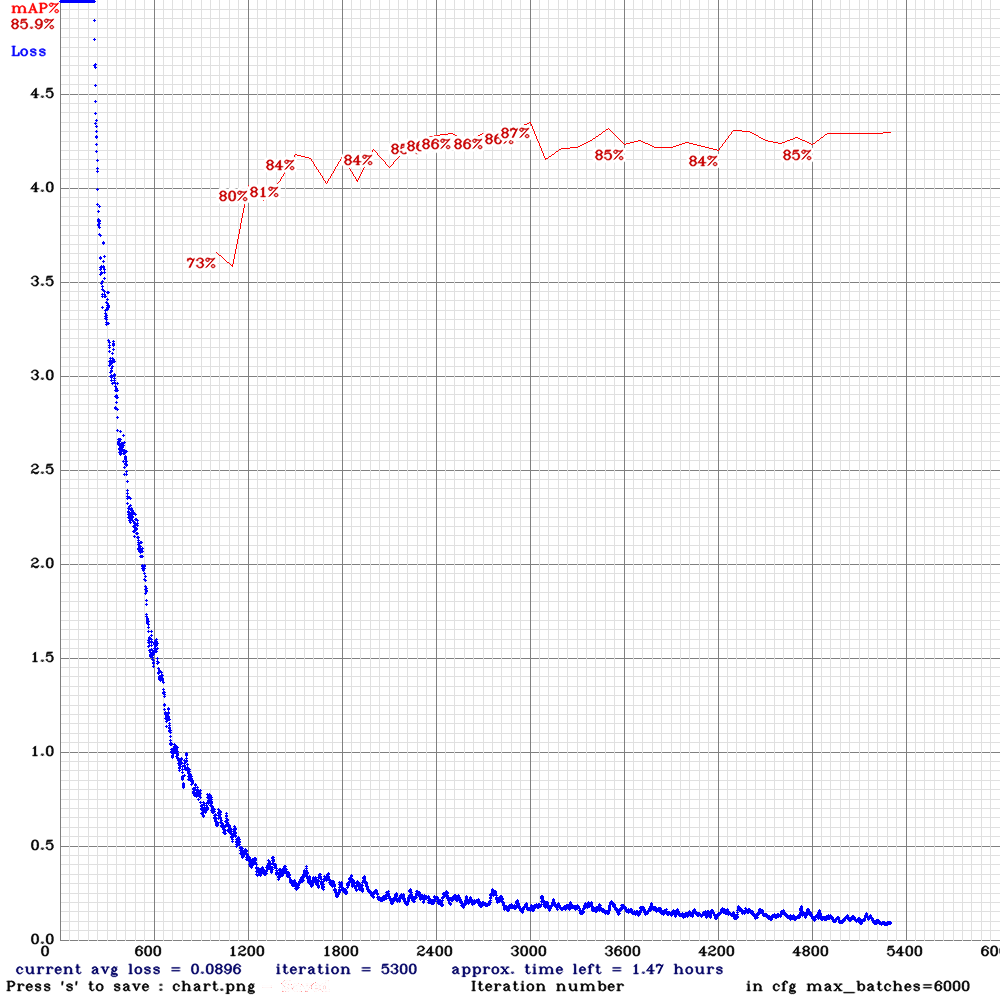
\includegraphics[width=0.4\textwidth]{pictures/painting_detection/training-v3.png}
    \caption{YOLOv3 trained on our custom dataset.}
    \label{fig:training-v3}
\end{figure}

\begin{figure}[h!]
    \centering
        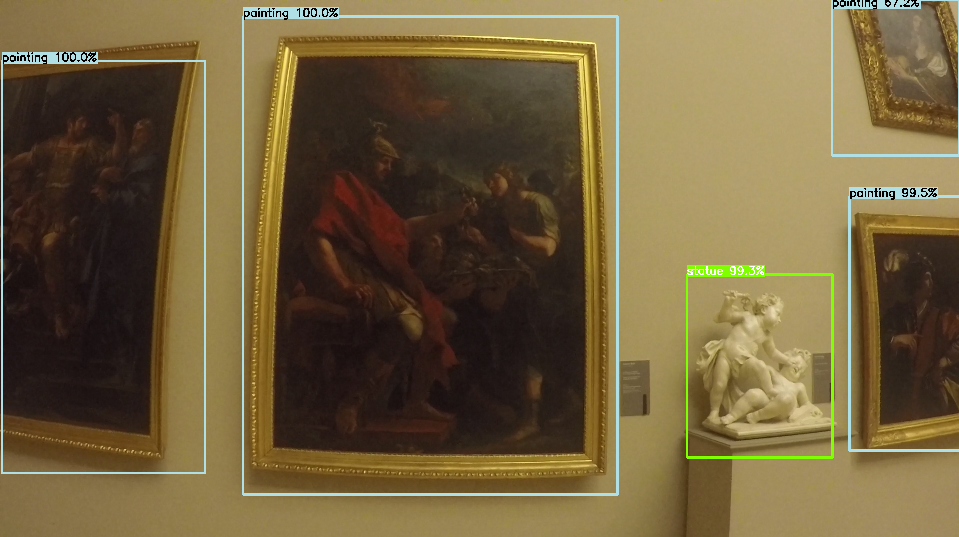
\includegraphics[width=0.45\textwidth]{pictures/painting_detection/yolo-detection2.PNG}
    \caption{Detection with YOLOv3.}
    \label{fig:yolo_detection}
\end{figure}


\begin{figure*}[h]
    \minipage{0.45\textwidth}
      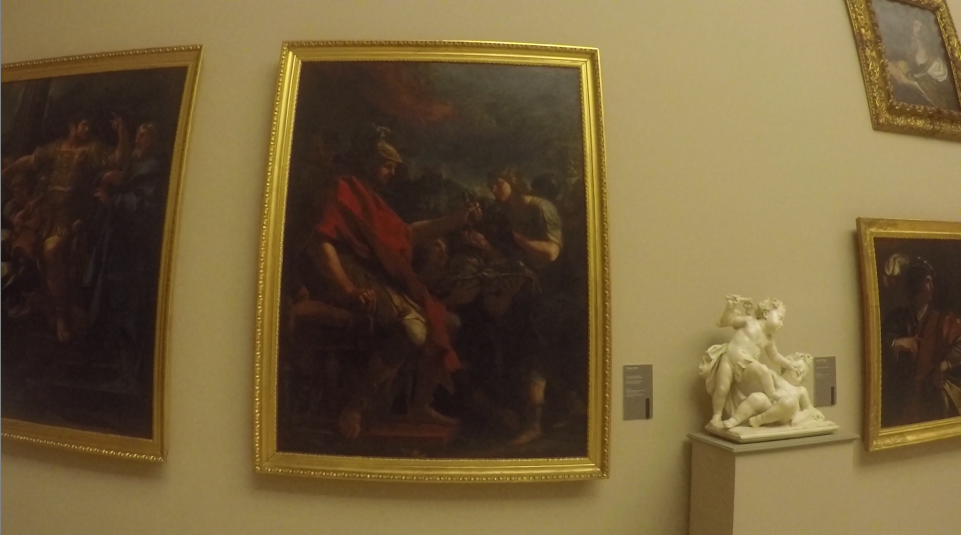
\includegraphics[width=\linewidth]{pictures/painting_detection/detection_withoutNN_1.PNG}
      \caption*{Image with shadow}\label{fig:shadow1}
    \endminipage\hfill
    \minipage{0.45\textwidth}
      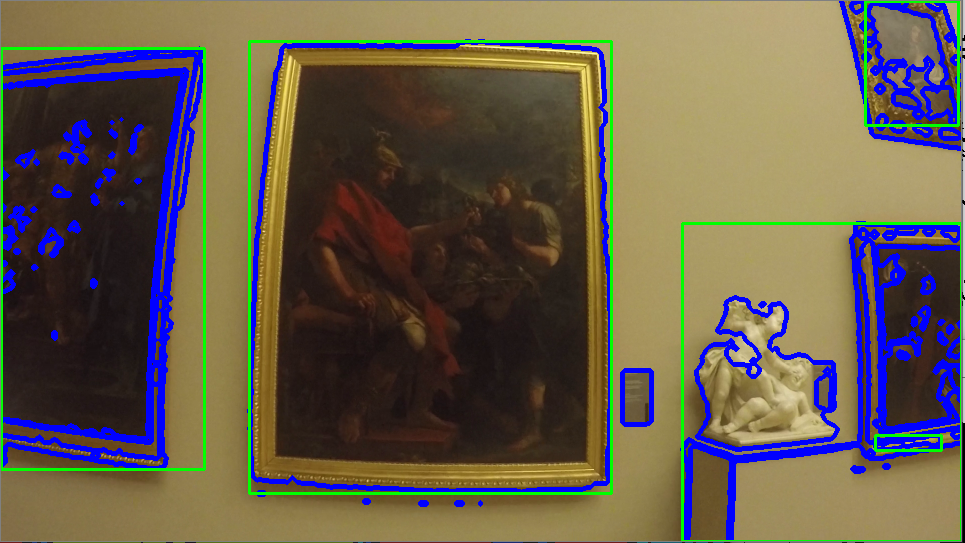
\includegraphics[width=\linewidth]{pictures/painting_detection/detection_withoutNN_3.PNG}
      \caption*{Not precise bounding box}\label{fig:shadow2}
    \endminipage\hfill
    \caption{Inaccurate detection.}\label{fig:innaccurate_detection}
\end{figure*}







The detection of paintings, statues and people is done through a custom YOLOv3 neural network~\cite{yolov3}.
Yolo is an architecture that provides a new approach to object detection, in which a single neural network predicts bounding boxes and class probabilities directly from full images in one evaluation.

In order to use this neural network we have labeled 1343 images, 805 of them have been used to train the network, 269 for the validation set and 269 for the test set, providing a total number of 3733 labels. The images of paintings and statues were taken from frames extracted by some videos recorded in the Galleria Estense, for the person class was instead used a mix of images taken from the previous videos and some images of people in another museum to increase generalization.
Fig.~\ref{fig:training-v3} shows the graph for the training that has been performed with darknet~\cite{darknet} in which we took the mAP every 1000 iterations in order to have the best weights that weren't affected by overfitting.

In the end we got a powerful neural network with high performance and capable of a good generalization, a result of the detection can be seen in fig.~\ref{fig:yolo_detection} while the performance is shown in tab.~\ref{tab:detection_performance}.

An important point is the data management: the train set, the validation set and the test set have been balanced with a 60/20/20 split, this allowed the network to have a better performance and to predict classes in a correct way.



\begin{table*}[ht!]
    \centering
\begin{tabular}{|c|c|c|c|c|}
\hline
\multicolumn{5}{|c|}{\textbf{Detection Performance}}       \\ \hline
\multicolumn{1}{|l|}{} & \textbf{Painting} & \textbf{Statue} & \textbf{Person} & \textbf{Overall} \\ \hline
\textbf{TP}        & 550     & 174     & 125     & 849     \\ \hline
\textbf{FP}        & 107     & 19      & 32      & 158     \\ \hline
\textbf{Precision} & 83,71\% & 90,16\% & 79,62\% & 84,31\% \\ \hline
\textbf{Recall}    & -       & -       & -       & 94\%    \\ \hline
\textbf{Average IoU}       & -       & -       & -       & 71\%    \\ \hline
\textbf{AP}        & 97,29\% & 98,61\% & 75,45\% & -       \\ \hline
\textbf{mAP}       & -       & -       & -       & 90,45\% \\ \hline
\end{tabular}
\caption{Detection performance with YOLOv3.}
    \label{tab:detection_performance}
\end{table*}



\subsubsection{Comparison with previous technique}
In a previous pipeline (showed in fig.~\ref{fig:pipeline_detection}) the detection was made without neural networks: the image was at first transformed in a gray level image, preprocessed with adaptive threshold, median blur \cite{median-blur} to remove the noise and opening, and then we computed the borders.
After the preprocessing, the pipeline uses the result to compute the Connected Component Labeling~\cite{Grana_ccl} to label the background and the foreground objects.
In order to label the foreground objects as paintings, the components needed to have an entropy grater than a threshold, and then the bounding boxes were drawn.

Despite this method worked well in some scenarios, it wasn't able to adapt to strong luminance variation, to manage the presence of shadows and to generalize with all the classes. As we can see in fig~\ref{fig:innaccurate_detection}, the two big paintings are correctly detected, while the statue and the lower right painting are merged in a single bounding box since their borders overlap. Many times the shadow was recognized as part of the painting and for this reason the IoU was not precise enough, this led us to choose the neural network approach.


\section{Painting Retrieval}
Painting retrieval uses ORB \cite{orb} keypoints detector and descriptor to find matches between two images. ORB, aka "Oriented FAST and Rotated BRIEF", is at two orders of magnitude faster than the old used SIFT \cite{sift} and this is the main reason why we have chosen to use this method, in order to achieve the painting retrieval with a good performance/results ratio.
\subsection{Improvements}
To improve the retrieval and to reduce false matches, we used the ratio test described in Lowe's paper \cite{sift}, in order to get the best matches. Given the two best matches (the best match and the second best match) for a keypoint, we define a \(threshold\) and if the ratio between the distance of the two best matches is below that ratio, we reject that match, considering it equivalent to noise and because the best match is too much similar to the second one. 

Our goal was to keep the number of paintings correctly found in the database high but at the same time, not decreasing the number of correctly not found paintings that are not in the database. We have chosen \(threshold = 0.6\) because increasing it even by just 0.1, although it decreased the number of positive answer to paintings not listed in the database, this resulted in an increasing number of wrong matches for the paintings in the database. Decreasing the threshold led to an opposite situation and both of the cases didn't meet our goal.

Computing the same keypoints and descriptors for the same paintings in the database has resulted in a slow start, causing the retrieval to wait a couple of seconds or more. Computing the keypoints and descriptors one time and storing them into a file, reduced the retrieval initialization by more than 40\%.
\subsection{Evaluation method}
To evaluate the retrieval, we tested it with a sample of 3 random frames per video, with a total of 100 randomly selected videos out of 208. Some of these frames either did not contain any frames or the region of interest of the paintings exceeded the frame size, therefore 100 frames out of the total of 300 were discarded. 266 are the total paintings detected using our trained model and 45 of these were discarded because they were unrecognizable, due to their small size and/or their brightness. 
For the remaining 221 paintings, we manually counted every time we saw a wrong or a right answer. More precisely, we checked if the painting was in the database and the retrieval answer, building the matrix in table \ref{tab:retrieval_eval}.

% Please add the following required packages to your document preamble:
% \usepackage{multirow}
% \usepackage[table,xcdraw]{xcolor}
% If you use beamer only pass "xcolor=table" option, i.e. \documentclass[xcolor=table]{beamer}
\begin{table}
\centering
\begin{tabular}{cccc}
 &
   &
  \multicolumn{2}{c}{\textit{Retrieval answer}} \\ \cline{3-4} 
 &
  \multicolumn{1}{c|}{} &
  \multicolumn{1}{c|}{\textbf{Found}} &
  \multicolumn{1}{c|}{\textbf{\begin{tabular}[c]{@{}c@{}}Wrong or\\ not found\end{tabular}}} \\ \cline{2-4} 
\multicolumn{1}{c|}{} &
  \multicolumn{1}{c|}{\textbf{In DB}} &
  \multicolumn{1}{c|}{\cellcolor[HTML]{34FF34}58} &
  \multicolumn{1}{c|}{\cellcolor[HTML]{FE0000}60} \\ \cline{2-4} 
\multicolumn{1}{c|}{\multirow{-3.5}{*}{\rotatebox[origin=c]{90}{\textit{Paintings}}}} &
  \multicolumn{1}{c|}{\textbf{Not in DB}} &
  \multicolumn{1}{c|}{\cellcolor[HTML]{FE0000}47} &
  \multicolumn{1}{c|}{\cellcolor[HTML]{34FF34}56} \\ \cline{2-4} 
\end{tabular}
\caption{Painting retrieval evaluation results}
\label{tab:retrieval_eval}
\end{table}
    
The result is that 58 out of 221 paintings were in the database and they were correctly retrieved from it, 56 out of 221 were not in the database but the retrieval correctly gave us a no match found. The remaining paintings are the ones that were wrongly retrieved from the database, 60, and the ones that had not an instance in the database but a wrong match was uncorrectly found.

Accuracy is the measurements used to get information on how good our configuration is: \[ Accuracy = \frac{58+56}{221} \approx 0.52 \]
We think that this result is pretty good, based on the fact that we could increase the real matched paintings reducing the uncorrectly found paintings that were not actually in the database, adding them manually to it.
\subsection{Painting Rectification}
We manage to perform a very accurate rectification when the painting retrieval is able to correctly fetch the painting entry from our database. In this case, not only we have the correct correspondence of paintings, but we can also exploit the descriptors obtained from ORB to compute an extremely accurate homography matrix, thanks to the large number of keypoints, to then compute the projective transformation.

\begin{figure}[h!]
    \centering
    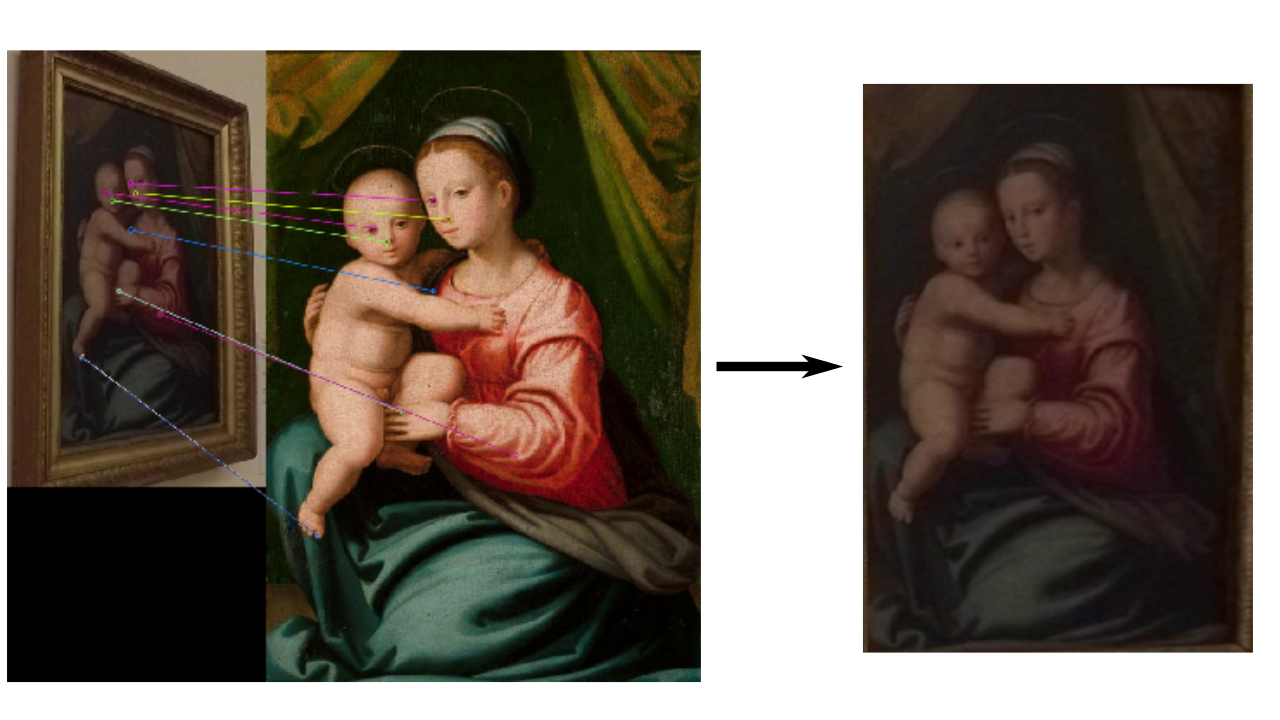
\includegraphics[width=.49\textwidth]{pictures/painting_rectification/rectification.png}
    \caption{example of painting rectification}
    \label{fig:rectification_ex}
\end{figure}

When the retrieval fails, for the lack of descriptors or when the painting is missing from the database, we use Harris Corner Detetor~\cite{harris-corner} to find the corners of the painting and use them as source points for our homography matrix. This method has a worse performance than the descriptors method, since the corners are not always precise.

\section{People Localization}
Our approach to achieve this task is based on the quality of the detection and painting retrieval. In fact, if our trained model correctly detect a person, in order to localize that person, we use informations about the paintings detected by the model and retrieved from the database.

\subsection{Evaluation}
We have access to the paintings\_db, with informations about the room where each painting is located, and this could make you think that our solution is optimal. Unfortunately, there are two main problems that worsen our evaluation:

\begin{enumerate}[label=\alph*)]
	\item \label{retrieval_case} The painting retrieval almost performs a random choice when a painting is in the database.
    \item \label{painting_other_room} We do not take into account the scenario in which the camera and the person are in a room, while a detected painting is in another room, visible through a door.
\end{enumerate}
\section{People Facing Paintings}

\subsection{3D Rectification}


\begin{figure*}[h]
    \minipage{0.45\textwidth}
      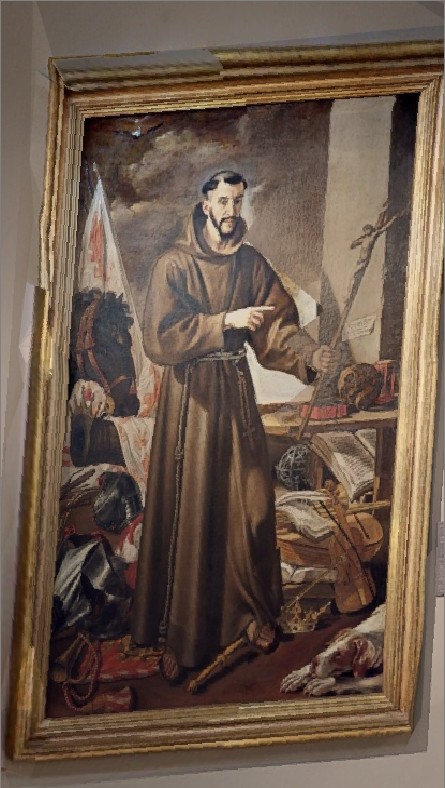
\includegraphics[width=\linewidth]{pictures/painting_detection/3d_rectification_original.PNG}
      \caption*{Original 3D model painting}\label{fig:rectification_original}
    \endminipage\hfill
    \minipage{0.45\textwidth}
      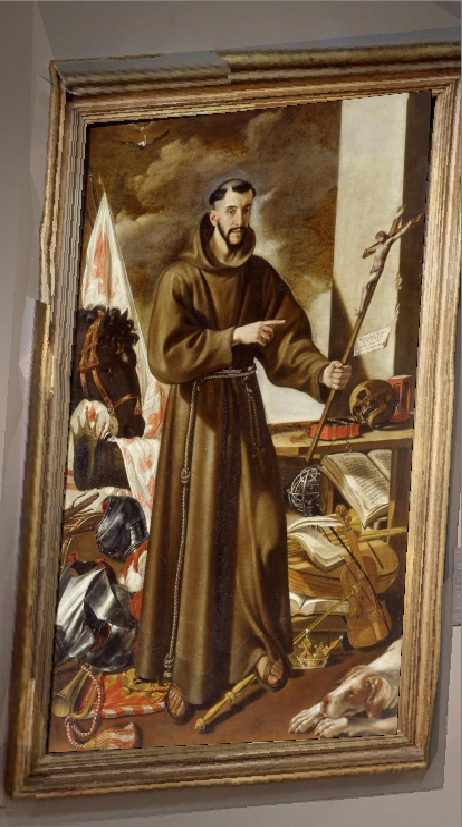
\includegraphics[width=\linewidth]{pictures/painting_detection/3d_rectification_warped.PNG}
      \caption*{Replaced painting}\label{fig:rectification_warped}
    \endminipage\hfill
    \caption{Rectification painting of 3D model}\label{fig:3d-warping}
\end{figure*}


The 3D Rectification is the last optional task that has been done. The scope was to replace the painting that was present in a 3D model with the same painting but with an higher resolution. Have been taken some screenshot of the 3D model with an off-line approach, then were extracted all the ROI that were present in the acquired image and each painting of the model was confronted with all the painting in our database. The painting identified was first warped with an homography trasformation in order to be in the same prospective of the painting in the screenshot and then was replaced with the previous one; in case of mismatch nothing was done. One of the results that has been achieved is showed in the fig.~\ref{fig:3d-warping}.


\printbibliography[heading=bibintoc,title={Bibliography}]\thispagestyle{empty}
\clearpage
\section*{Additional Resources}

\begin{figure}[h!]
  \centering
    \resizebox{0.6\textwidth}{!}{
      \minipage{0.3\textwidth}
        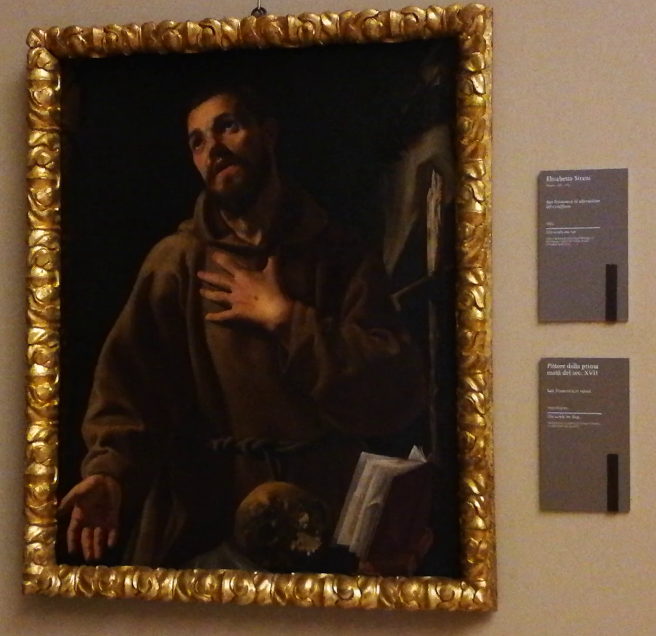
\includegraphics[width=\linewidth]{pictures/painting_detection/Frame.png}
        \caption*{Frame from video}\label{fig:Frame}
      \endminipage\hfill
      \minipage{0.3\textwidth}
        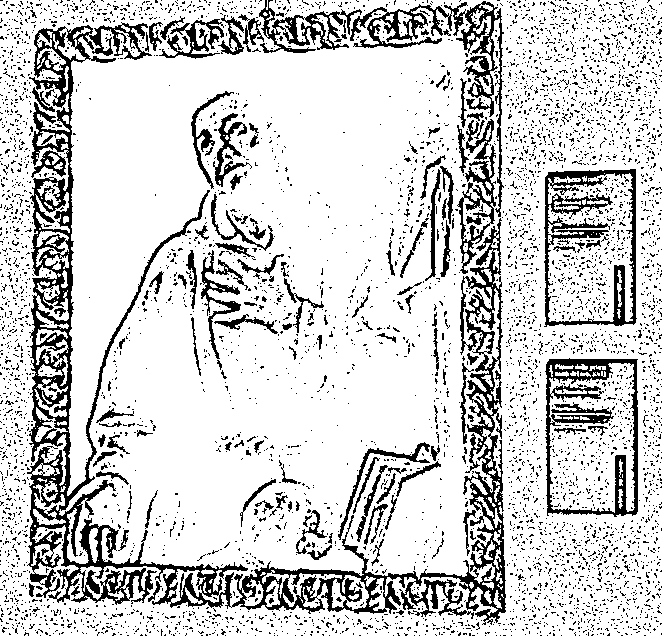
\includegraphics[width=\linewidth]{pictures/painting_detection/2-adaptive_threshold.PNG}
        \caption*{Adaptive threshold}\label{fig:adaptive_threshold}
      \endminipage\hfill
      \minipage{0.3\textwidth}%
        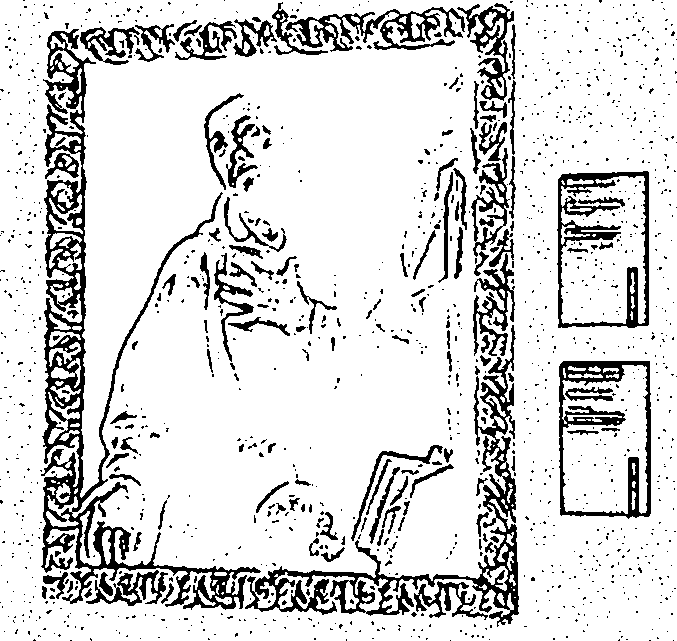
\includegraphics[width=\linewidth]{pictures/painting_detection/3-median_blur.PNG}
        \caption*{Median blur}\label{fig:median_blur}
      \endminipage}

      \resizebox{0.6\textwidth}{!}{
      \minipage{0.3\textwidth}
        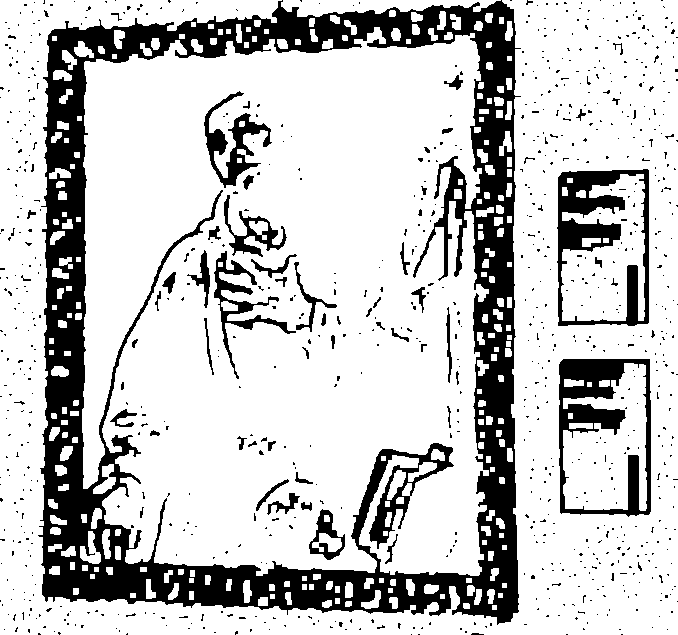
\includegraphics[width=\linewidth]{pictures/painting_detection/4-opening.PNG}
        \caption*{Opening}\label{fig:opening}
      \endminipage\hfill
      \minipage{0.3\textwidth}
      \captionsetup{font=small}
        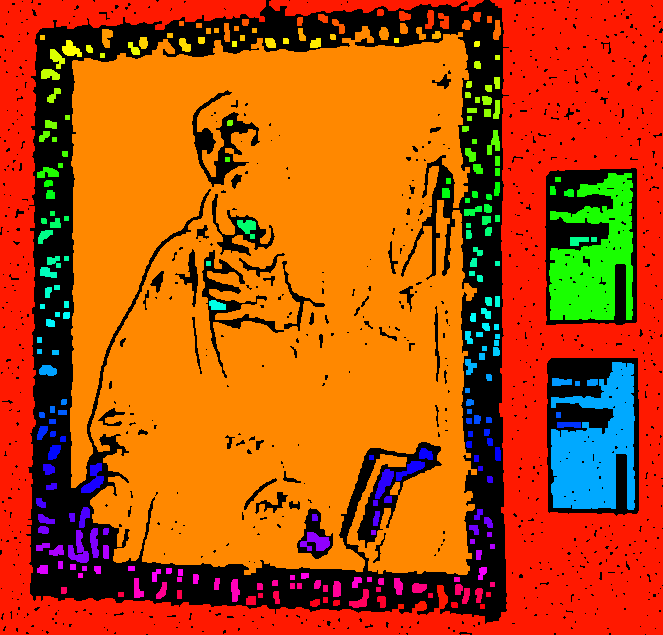
\includegraphics[width=\linewidth]{pictures/painting_detection/5-ccl.PNG}
        \caption*{Connected Component Labeling}\label{fig:ccl}
      \endminipage\hfill
      \minipage{0.3\textwidth}%
        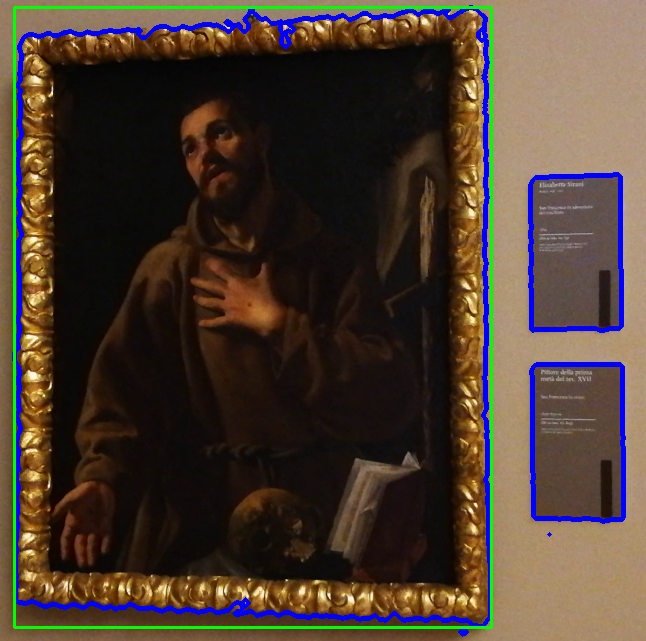
\includegraphics[width=\linewidth]{pictures/painting_detection/6-bbox.PNG}
        \caption*{Painting Detection}\label{fig:bbox}
      \endminipage}
      \caption{Detection pipeline without neural network.} \label{fig:pipeline_detection}
  \end{figure}


\end{document}
